\documentclass{article}\usepackage[]{graphicx}\usepackage[]{color}
%% maxwidth is the original width if it is less than linewidth
%% otherwise use linewidth (to make sure the graphics do not exceed the margin)
\makeatletter
\def\maxwidth{ %
  \ifdim\Gin@nat@width>\linewidth
    \linewidth
  \else
    \Gin@nat@width
  \fi
}
\makeatother

\definecolor{fgcolor}{rgb}{0.345, 0.345, 0.345}
\newcommand{\hlnum}[1]{\textcolor[rgb]{0.686,0.059,0.569}{#1}}%
\newcommand{\hlstr}[1]{\textcolor[rgb]{0.192,0.494,0.8}{#1}}%
\newcommand{\hlcom}[1]{\textcolor[rgb]{0.678,0.584,0.686}{\textit{#1}}}%
\newcommand{\hlopt}[1]{\textcolor[rgb]{0,0,0}{#1}}%
\newcommand{\hlstd}[1]{\textcolor[rgb]{0.345,0.345,0.345}{#1}}%
\newcommand{\hlkwa}[1]{\textcolor[rgb]{0.161,0.373,0.58}{\textbf{#1}}}%
\newcommand{\hlkwb}[1]{\textcolor[rgb]{0.69,0.353,0.396}{#1}}%
\newcommand{\hlkwc}[1]{\textcolor[rgb]{0.333,0.667,0.333}{#1}}%
\newcommand{\hlkwd}[1]{\textcolor[rgb]{0.737,0.353,0.396}{\textbf{#1}}}%
\let\hlipl\hlkwb

\usepackage{framed}
\makeatletter
\newenvironment{kframe}{%
 \def\at@end@of@kframe{}%
 \ifinner\ifhmode%
  \def\at@end@of@kframe{\end{minipage}}%
  \begin{minipage}{\columnwidth}%
 \fi\fi%
 \def\FrameCommand##1{\hskip\@totalleftmargin \hskip-\fboxsep
 \colorbox{shadecolor}{##1}\hskip-\fboxsep
     % There is no \\@totalrightmargin, so:
     \hskip-\linewidth \hskip-\@totalleftmargin \hskip\columnwidth}%
 \MakeFramed {\advance\hsize-\width
   \@totalleftmargin\z@ \linewidth\hsize
   \@setminipage}}%
 {\par\unskip\endMakeFramed%
 \at@end@of@kframe}
\makeatother

\definecolor{shadecolor}{rgb}{.97, .97, .97}
\definecolor{messagecolor}{rgb}{0, 0, 0}
\definecolor{warningcolor}{rgb}{1, 0, 1}
\definecolor{errorcolor}{rgb}{1, 0, 0}
\newenvironment{knitrout}{}{} % an empty environment to be redefined in TeX

\usepackage{alltt}
\usepackage{hyperref}

\title{Introducing \LaTeX and Sweave}
\author{Marc and Kyle}
\IfFileExists{upquote.sty}{\usepackage{upquote}}{}
\begin{document}


\maketitle

%\tableofcontents

\section{What is \LaTeX?}

\LaTeX is an open source word processor that produces high quality documents. In addition, R commands can be integrated into text to  `weave' data analysis, graphics, and text into a professional finished product.

\subsection{Why use \LaTeX?}

TBD

\section{Using R Studio}

Before using \LaTeX, we need to define how files are 'knited' to create pdf files. After starting R studio, choose the  `Tools' menu item and select global options. On the left, select the `Sweave' option and make sure the default values match Figure~\ref{fig:sweave}. 

\begin{figure}{h}
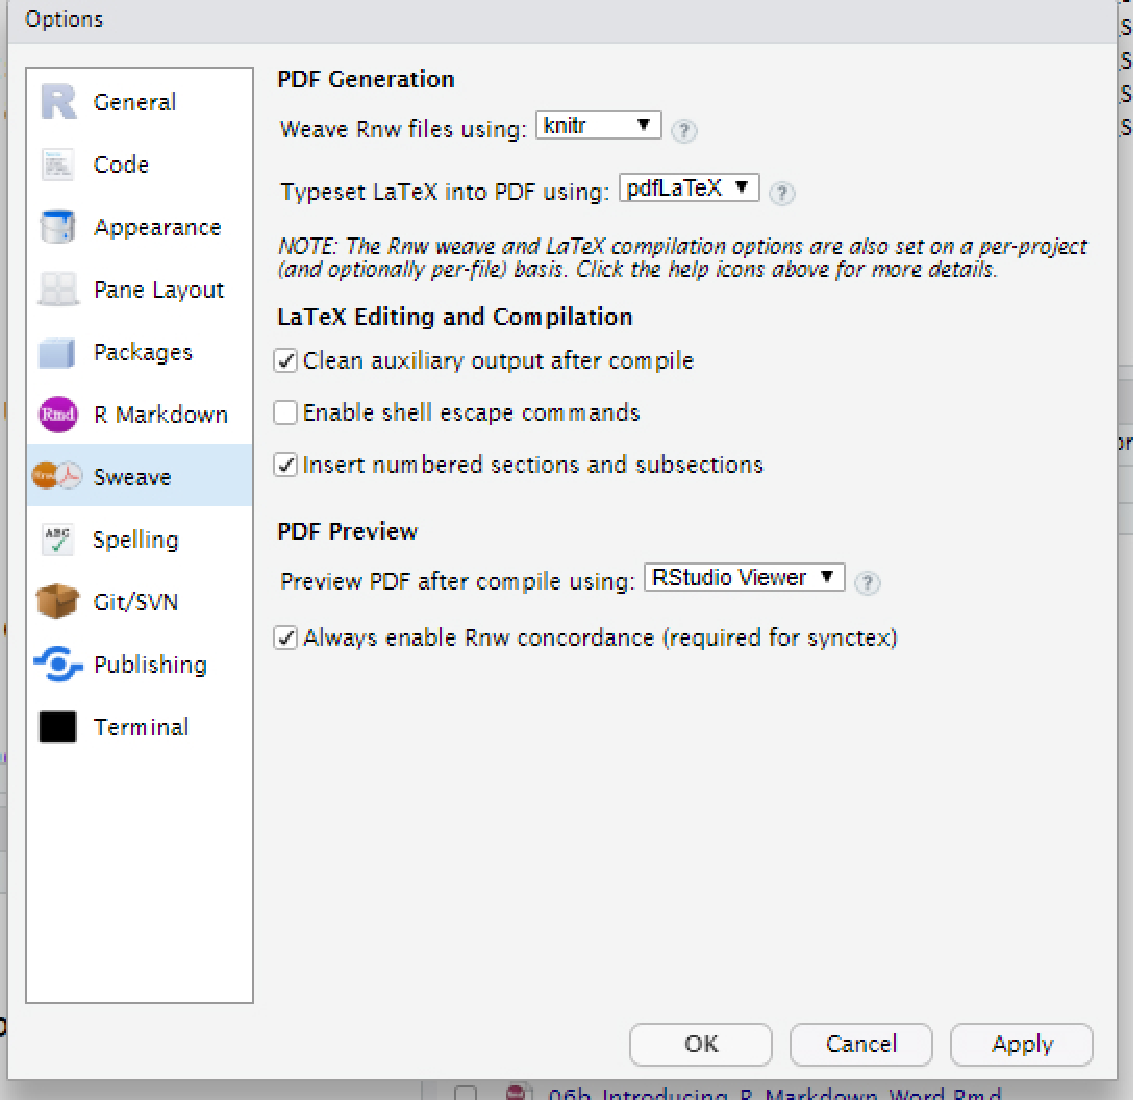
\includegraphics[width=\textwidth]{graphics/Sweave_setup}
\caption{Sweave setup screen shot}
\label{fig:sweave}
\end{figure}

\section{Creating \LaTeX~Documents}

\subsection{Document Structure: Preamble}

We usually declare the type of document on the first line of the text file, using the command \verb!\documentclass{}!. Inside the curly brackets we specify the type of document that you want, e.g. article, letter, book, minimal, or memoir. In general, I recommend you begin with article.

\subsection{Title and Author}

The author and title are specified in the preamble with the following commands:

\medskip
\noindent\verb!\title{This is my title}!

\noindent\verb!\author{This is the author or list of authors}!

\subsection{Begin and End}

Special blocks are developed within \verb!\begin{}! and \verb!\end{}! commands. For every block, both the begin and end must be present or you will generate errors.

In fact, after the preamble, the documents text is initiated by the \verb!\begin{document}! and ends at \verb!\end{document}!.

\subsection{Printing the Title and Author}

After the \verb!\begin{document}! is a good time to print the title, author and date of the pdf, which is all done with a \verb!\maketitle! command. 


\subsection{Sections and Subsections}

Each section and subsection (and subsubsection) heading are hierarchically defined and specified with the following commands:


\medskip
\noindent\verb!\section{This is a section heading}!

\noindent\verb!\subsection{This is a subsection heading}!

\noindent\verb!\subsubsection{This is a subsubsection heading}!

\bigskip
Please note, if you define a section, there must be more than one. Similary, if you create a subsection, be sure that it's not alone in the section -- otherwise, why have the break at all!

Finally, try to avoid putting text between dropping down into categories. In other words, don't insert a paragraph between a section and a subsection. Define the subsection so that the paragraph is applicable to the subsection and the section. 

\subsection{Special Characters that Cause Problems}

Most special characters are reserved for \LaTeX type setting -- see table for some important ones. These often create errors for beginners and experienced users alike, but for beginners the frustration generated by these errors can be overwhelming!

Review Table \ref{tab:specialcharacters} to appreciate some of these characters (Table \ref{tab:specialcharacters}).

\begin{table}
\caption{Write a Caption here.}
\label{tab:specialcharacters}
\begin{tabular}{cp{6cm}p{6cm}}\hline
Character   & Type Setting Function & Associated Error \\ \hline\hline
\%          & Percent symbols used to make comment lines and are not printed when compiled.& If you want to print the percent symbol, use \verb!\%! \\
\&          & Ambersands are used for tab in tables& When used outside the table environment, you'll get errors, use \verb!\&! if you want to use the symbol in writing.\\
\$          & Dollar symbols are use to create 'math' mode blocks, for example if you want to use the Greek letter $\alpha$, \verb!$\alpha$! & If you really want a dollar sign, then you'll want to use \verb!\$!.\\
\hline
\end{tabular}
\end{table}

If you are trying to use the characters in the text, then put a backslash in front of them. If you are using them in a type-setting capacity, you should look up how to use them online.

The symbol issues listed above are relatively easy to address. The more difficult problem is if you non-ascii characters creap into the document. The issues usually arises when we past in text form word or google docs, where quotes (`` and '') or dashes (-, \textemdash) or funky letters or symbols ($\alpha$, $\chi^2$, \~{n}) are used. We can specify these in \LaTeX, but not pasting in these characters directly into the Rnw file. 

\section{Integrating R Commands with Sweave}

\subsection{Compile PDF workflow}

Now the best part of using \LaTeX and rstudio is that you can create text that runs the R code as you compile and even use the results in the text.

We begin with an Rnw File. When we `Compile PDF', Rstudio routes the file through a Sweave processe to create a \TeX file. The \TeX file is then compiled into a pdf.

\begin{center}
Rnw $->$ TeX $->$ PDF
\end{center}

\subsection{R Chunks}

R chunks or blocks are delineate with the following code:

\bigskip
\noindent \verb!<<>>=! 

\noindent ... R code stuff

\noindent \verb!@!

\bigskip
Within the less than and greater than sybols, one can customize how the R block is processed. For more information, one should see other more detailed resources.



\subsection{Creating Figures}

We intiate figures with \verb!\begin{figure}! and ends with \verb!\end{figure}!. For more information, the reader is directed to one of several online resources on R and \LaTeX.

\subsection{Creating Bibliography}

To create a bibliography, we need to add some packages, for example, \verb!\usepackage{natbib}! into the preamble. We also make sure the bibliographic style is defined for the Council of Scientific Editors by making sure the cbe.bst file is in the home directory. 

To cite in text you can use one of two commands \verb!\citep{}! and \verb!\citet{}!. Inside you curly brackets you use the citation 'key' to reference each citation. Finally you'll add \verb!\bibliographystyle{cbe.bst}! and \verb!\bibliography{bibtexfile}! just before the \verb!\end{document}! line.

\section{Minium Working Document}

I have created a minimum working document and sample bib file that you can upload to R studio server, save with a new name and compile. If it compiles correctly, you are on your way. 

Here are the URLs:

\smallskip
\noindent \url{https://github.com/marclos/Climate_Change_Narratives/blob/master/Communication_Resources/Lab_Report_Template.Rnw}

\medskip
\noindent \url{https://github.com/marclos/Climate_Change_Narratives/blob/master/Communication_Resources/bibexample.bib}

\medskip
\noindent \url{https://github.com/marclos/Climate_Change_Narratives/blob/master/Communication_Resources/cbe.bst}

Be sure to upload all three files or you won't be able to compile the document.

\end{document}
